\title{Computational Neurophysiology - Final Project}
\author{Ryan Spangler}
\date{\today}

\documentclass[12pt]{article}

\usepackage{commath}
\usepackage{graphicx}
\usepackage{listings}

% python highlighting ----------
\usepackage{color}
\usepackage{listings}
\usepackage{textcomp}
\usepackage{setspace}
%\usepackage{palatino}

\renewcommand{\lstlistlistingname}{Code Listings}
\renewcommand{\lstlistingname}{Code Listing}
\definecolor{gray}{gray}{0.6}
\definecolor{green}{rgb}{0.1,0.6,0.3}
\definecolor{orange}{rgb}{0.9,0.7,0.1}
\definecolor{blue}{rgb}{0,0.6,0.8}

\lstnewenvironment{python}[1][]{
\lstset{
language=python,
basicstyle=\ttfamily\footnotesize\setstretch{1},
stringstyle=\color{red},
showstringspaces=false,
alsoletter={1234567890},
otherkeywords={\ , \}, \{},
keywordstyle=\color{blue},
emph={access,and,break,class,continue,def,del,elif,else,%
except,exec,finally,for,from,global,if,import,in,is,%
lambda,not,or,pass,print,raise,return,try,while},
emphstyle=\color{gray}\bfseries,
emph={[2]True, False, None, self},
emphstyle=[2]\color{orange},
emph={[3]from, import, as},
emphstyle=[3]\color{blue},
upquote=true,
morecomment=[s]{"""}{"""},
commentstyle=\color{gray}\slshape,
emph={[4]1, 2, 3, 4, 5, 6, 7, 8, 9, 0},
emphstyle=[4]\color{blue},
literate=*{:}{{\textcolor{blue}:}}{1}%
	{=}{{\textcolor{blue}=}}{1}%
	{-}{{\textcolor{blue}-}}{1}%
	{+}{{\textcolor{blue}+}}{1}%
	{*}{{\textcolor{blue}*}}{1}%
	{!}{{\textcolor{blue}!}}{1}%
	{(}{{\textcolor{blue}(}}{1}%
	{)}{{\textcolor{blue})}}{1}%
	{[}{{\textcolor{blue}[}}{1}%
	{]}{{\textcolor{blue}]}}{1}%
	{<}{{\textcolor{blue}<}}{1}%
	{>}{{\textcolor{blue}>}}{1},%
    frame=fullbox, rulesepcolor=\color{gray},#1
%framexleftmargin=1mm, framextopmargin=1mm, frame=shadowbox, rulesepcolor=\color{blue},#1
}}{}

\setcounter{secnumdepth}{0}

\begin{document}
\maketitle

\section{Introduction}

The role of synchronization in the binding of perception has slowly come into appreciation over the last couple decades.  That synchronization is a widespread and fundamental aspect of neural behavior is not disputed \cite{Buzsaki}.  What is disputed is what exactly the role of synchronization is.  One proposal is that synchronization binds together otherwise independent perceptual features, symbolizing in a way that these features ``belong'' together in the current perceptual landscape \cite{Melloni}.  

The physical mechanism for consciousness is still unknown, but that has not stopped several researchers from searching for what they call ``neuronal correlates to consciousness'', or NCC \cite{Rees}.  Regardless of whether they can explain what exactly is happening, they can say that when a subject claims to experience a conscious percept, there is a corresponding and measurable activity of some variety in the nervous system.  One of the most compelling NCC is that of transient synchronization of neural assemblies in the cortex.  One question from all this is: why synchronization?  How does synchronization in particular help the cortex to perceive whole things, when these perceptions are composed of more or less atomic features?  

One way to approach this problem is to start with basic models of synchronization.  How can synchronization be usefully modeled in a way that is applicable to neural dynamics?  We explore a simple model of synchronization, the Kuramoto model, and then one of its applications to the connectivity and function of the primary visual cortex, given by Sompolinsky \cite{Sompolinsky}.  Ultimately we will elaborate on the Sompolinsky model by providing a means of differing connection topologies between receptive fields, and varying dimensions of sensory stimuli.

\section{Models of Synchronization}

\subsection{Kuramoto Model}

One of the most successful models of general mathematical synchronization is the Kuramoto model \cite{Acebrón} \cite{Ermentrout}.  The $N$ elements in the Kuramoto model are simple phase oscillators with a single phase variable $\theta$ and a preferred frequency $\omega$.  In addition, there is a connection matrix $K$ whose elements $K_{ij}$ express the strength of the coupling between the $i$th element to the $j$th element.  The equation as a whole is given by a differential equation for a given element $i$:

$$ \od{\theta_i}{t}=\omega_i+\sum\limits_{j=1}^N K_{ij}\sin(\theta_j-\theta_i)$$

where $i=1,...,N$.  So basically, this equation is a sum over the sine of all of the differences between a particular element and all of the other elements, scaled by the connection matrix.  The sine plays the functional role of emphasizing the differences between the phases.  The more different are the phases of each of the oscillators to the one in question, the more that element's phase $\theta_i$ will be adjusted.  If all of the elements happen to be in the same phase then the summing term would vanish and we would be left with the $\omega_i$, which is the element's natural frequency.  Left entirely to its own devices, the phase $\theta_i$ would be adjusted by its natural frequency $\omega_i$ each time step, and the phase would march merrily along a constant cycle.  

The Kuramoto model displays remarkable robustness of synchronization, and if no other factors come into play the elements will be swiftly phase-locked.  This model is straightforward to implement.  Here is the python code for a basic implementation of the Kuramoto model:

\begin{python}[]
from pylab import *
tau = 2 * pi

class Kuramoto:
    def __init__(self, N, K=0.1, order=0.1):
        self.N = N
        self.K = K
        self.order = order
        self.scale = K / N
        self.reset()

    def reset(self):
        self.phase = random(self.N) * tau
        self.intrinsic = random(self.N) * self.order
        self.spikes = zeros(self.N)
        self.phases = self.phase

    def deltax(self, x):
        differences = sum(sin(self.phase - self.phase[x]))
        return self.intrinsic[x] + self.scale * differences

    def delta(self):
        return array(map(lambda x: self.deltax(x), range(self.N)))

    def step(self):
        self.phase += self.delta()
        spiking = (self.phase >= tau)
        self.spikes = vstack([self.spikes, where(spiking, 1, 0)])
        self.phase = where(spiking, self.phase - tau, self.phase)
        self.phases = vstack([self.phases, self.phase])

    def run(self, steps):
        self.reset()
        for step in range(steps):
            self.step()
\end{python}

To use this code it is necessary to have a working installation of python with pylab (python's open source incarnation of matlab), then for $N=50$ elements running for 100 time steps invoke:

\begin{python}
from kuramoto import *
model = Kuramoto(50)
model.run(100)
plot(model.phases)
\end{python}

This is a direct implementation of the above equations for the Kuramoto model.  N is the number of elements and K is a universal connection factor (all elements are coupled equally to one another). For this simulation the intrinsic frequencies are generated as random variables between 0.0 and 0.1, and the initial phase for each oscillator is somewhere between $0$ and $2\pi$.  The behavior is striking:

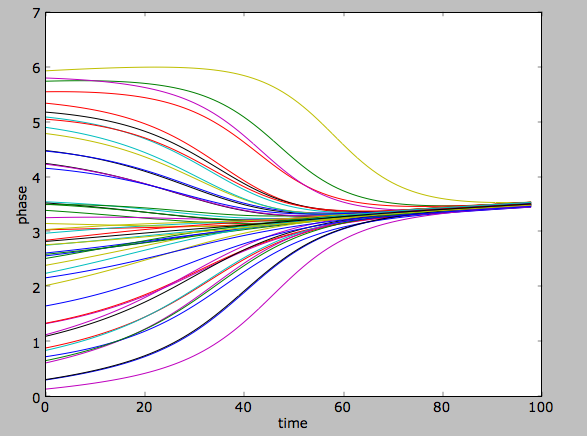
\includegraphics[scale=0.67]{kuramoto.png}

This is a plot of the phase of each element against time.  In the space of about 100 time steps the model was completely synchronized.  It can synchronize even more quickly if $K$ (the coupling) is raised.  What else is remarkable is that each of these oscillators has a different innate phase, and the system seeks a common frequency that is a balance of all of the elements at once.  Here is the same model at 300 time steps to emphasize the strengh of the synchronization.

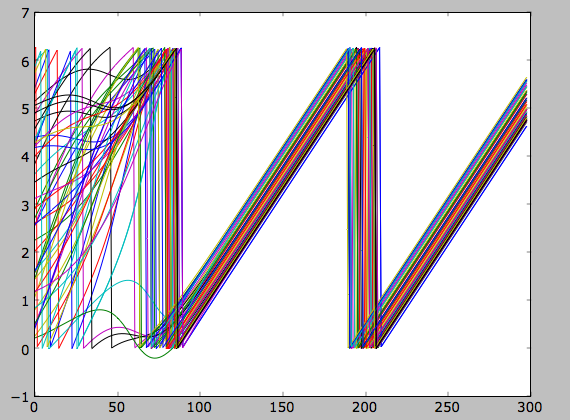
\includegraphics[scale=0.67]{synchronization.png}

\section{Synchronization and the Visual System}

One of the neural systems we know quite a bit about is the primary visual cortex, the initial gateway of direct visual information into the cortex \cite{Tanaka}.  There are findings that reveal potential mechanisms for perception based on synchronization between populations of coordinating neural groups.  Some of these findings are nicely summarized by \cite{Sompolinsky}.  The subject of Sompolinsky's work is the orientation of bars that span a receptive field and the responsiveness of various neural assemblies in the presence of these bars.  A receptive field Sompolinsky defines to be a set of neurons that discriminate different features of the same spatial area.  These receptive regions are spatially vaguely defined, but are mostly circular and include much overlap with neighboring regions.  Within a receptive field the neurons each respond to a different stimulus.  One responds to horizontal bars say, and others vertical ones, with a spectrum of various angles in between.  Some code for red, some for green.  Some are responsive to motion in one direction, some motion in another (motion alone can be decomposed into direction, speed, rotation or expansion/contraction).  All of these neurons belonging to a common receptive field are clustered together, each firing fairly specifically to a single modality and a single flavor of that modality, but interacting with each other through synaptic coupling.  If there is a vertical bar that is green for example, the neurons that fire when there is only a vertical bar will synchronize with the neurons that fire in response to green.  This synchrony between mutually activated neurons is characteristic of activity within a receptive field.  

In addition to this action {\em within} a receptive field, there is also action {\em between} receptive fields.  This takes the character of synchronization between neurons which discriminate the same feature, but in neighboring receptive fields.  If the same vertical bar is detected in the neighboring field both vertical bar neurons will synchronize.  If the bar is broken, each vertical bar neuron will fire, but they may not synchronize.  Synchronization between receptive fields is accomplished through a system of weak coupling between corresponding neurons of similar sensitivity, whereas the coupling between neurons within a field are strongly coupled.  

All of this points to the functional role of synchronization in neural and cortical bases of perception.  Now that we know that synchronization is an important mechanism in the generation of experience, this leads to the question: how can synchronization be modeled?

\subsection{Sompolinsky's Model}

The Kuramoto model is impressive due to its strength of synchronization and its ultimate simplicity.  It is the perfect ingredient to more complex models, as is amply displayed in \cite{Acebrón}.  One of the intriguing applications of the Kuramoto model is Sompolinsky's work on the primary visual cortex \cite{Sompolinsky}.  This model attempts to capture the notion of interacting receptive fields discussed earlier.  Each neuron in the receptive field responds strongly to a single variety of a single type of stimulus, ignoring all others.  All of the neurons within a receptive field code for a different stimulus, but this pattern of selectivity is repeated in each neighboring receptive field, so that there is in a sense a mirror image, or tiling, of the selectivities in each field.  The neurons which respond to a particular feature are weakly coupled between receptive fields.  

To model this Sompolinsky used a system based on the simplified Kuramoto model above, but with variable coupling strengths between neurons to represent the different receptive fields, and the notion of a stimulus and a tuning curve for each neuron representing its responsiveness to that stimulus.  Neurons within a cluster each respond to a different stimulus according to a tuning curve, and activated neurons are coupled strongly and can be considered to reduce to the simple Kuramoto model.  Neurons between clusters are coupled if they respond to the {\em same} stimulus.  

Another addition is that the firing of a neuron is taken to be a probabilistic event.  In concrete terms, the firing probability $P$ of a neuron is given by 

$$ P(\mathbf{r},t)=V(\mathbf{r})(1+\lambda\cos\Phi(\mathbf{r},t)) $$

where $\Phi(\mathbf{r},t)$ is the phase of neuron $\mathbf{r}$ at time $t$, $\lambda$ is the strength of the contribution of the other neurons to a particular neuron's phase, and $V(\mathbf{r})$ is that neuron's response to the stimulus presented:

$$ V(\mathbf{r})=V(\theta_0(\mathbf{r})-\theta(\mathbf{r})) $$

Here, $\theta_0(\mathbf{r})$ is an angle representation of the stimulus at neuron $\mathbf{r}$, and $\theta(\mathbf{r})$ is that neurons own preferred angle.  The tuning curve used is 

$$ V(\theta_0(\mathbf{r})-\theta(\mathbf{r}))=e^{-|\theta_0(\mathbf{r})-\theta(\mathbf{r})|/\sigma} $$

where $\sigma$ is some scaling constant.  This tuning curve is a sharp point at the selectivity orientation with exponential decay in both directions from that point.  The behavior of the phases $\Phi$ of the system is almost exactly that of the Kuramoto model (with an extra noise term $\eta$ added):

$$ \tau_0\od{\Phi(\mathbf{r},t)}{t}=\omega\tau_0+\eta(\mathbf{r},t)-\sum\limits_{r'}J(\mathbf{r},\mathbf{r}')\sin(\Phi(\mathbf{r},t)-\Phi(\mathbf{r'},t)) $$

The $\theta$s in the original model have been replaced with the phase function $\Phi$ and the noise term $\eta$ has been introduced, which is governed by white noise with variance proportional to $\tau_0$.  The function $J(\mathbf{r},\mathbf{r'})$ has replaced the matrix $K$ to represent the connectivity of the neurons to each other.  This function $J(\mathbf{r},\mathbf{r'})$ is crafted in such a way as to express the connectivity scheme as outlined above, namely, neurons are strongly coupled to other neurons in their same receptive field, and weakly coupled to neurons in other receptive fields that display the same selectivity as themselves.  

Officially, the form of $J(\mathbf{r},\mathbf{r'})$ is

$$ J(\mathbf{r},\mathbf{r'})=V(\mathbf{r})W(\mathbf{r},\mathbf{r'})V(\mathbf{r'}) $$

where the $V$ terms represent the activity of each neuron and $W$ is the connections matrix.  This means that if either of the neurons are inactive the effect will be greatly reduced.  For any real effect to take place, both neurons must be active at the same time.  

The function $W_{RR}(\theta,\theta')$ is different depending on whether the neurons occupy the same receptive field or different ones.  For neurons in the same field, $W$ is simply

$$ W_{RR}(\theta,\theta')=\frac{W_S}{N} $$

where $W_S$ is the weighting constant for short range.  For neurons coding the same features in different receptive fields the relationship is

$$ W_{RR'}(\theta,\theta')=\frac{W_L}{N^2}F(\theta-\theta') $$

where $F(\theta-\theta')$ is a function which ensures that the difference between selectivities of coupled neurons is small.  

\section{Simulation}



\section{Discussion}



\bibliographystyle{plain}
\bibliography{final}

\end{document} 



